\subsection{基于神经网络的推荐算法}
\subsubsection{优势与局限}

近年来,深度学习技术被广泛应用于推荐系统中。
相较于传统机器学习方法,其优势在于:

\begin{itemize}
    \item 能够提取数据中非线性关系。这通常由Relu,sigmoid等非线性的激活函数完成。通过改变激活函数的选择和组合,模型可以拟合任何连续函数\cite{hornik1989multilayer},因此它能够捕捉到用户/物品之间更加深层与复杂的关系,具有更强的表征能力。
    \item 能够端到端地学习潜在解释因子与表征。它不需要手工设计特征,同时异构的内容信息(如文本、图片、视频等)可以通过不同的网络来提取出来,同时进行训练,能够有效地利用多模态的信息。如今,社交媒体的广泛普及,提供了大量多媒体的数据,而基于神经网络的推荐系统模型相较传统方法,在利用这些数据上,过程更加简单,效果也更好。
    \item 能够提供序列化任务的有效解决方案。RNN、CNN以及其他基于它们的模型,在序列化任务(如自然语言理解、语音识别等)上能取得更好的效果。在推荐系统中,序列化处理对于用户长短期行为分析、产品变革研究而言十分重要。
\end{itemize} 

相较于传统机器学习方法, 其局限在于:
\begin{itemize}

    \item\textbf{ 解释性。}神经网络表现得如同一个黑盒子,当人们需要寻求推荐的合理性时,神经网络难以给出其推导过程与解释。对于解释性要求较高的领域,基于神经网络的推荐系统并不是好的解决方案。
    \item \textbf{数据要求。}神经网络需要足够的数据进行训练,以得到有效的参数。在一些领域中,基于神经网络的推荐算法面临数据集样本量少、数据稀疏、冷启动等问题。
    \item \textbf{超参调整。}神经网络通常具有更多的超参,例如学习速率、正则项系数等。而超参的选择对于神经网络的最终预测效果可能有显著的影响。
\end{itemize}

认清神经网络相较于传统算法的优势与局限是十分重要的,当下许多基于神经网络的推荐算法,贡献就在于克服其劣势且充分发挥其优势。如为了减轻超参调整的复杂性与解释性问题,近期一篇论文\cite{tay2018latent}对传统的metric learning 方法进行拓展,添加了注意力机制,同时只引入一个超参。

\subsubsection{基本模型}
基于神经网络的推荐算法,大多是对基本模型进行扩展或组合。
基本模型主要包括:
\begin{itemize}
    \item \textbf{多层感知机(MLP)}。层层之间全连接,因此参数很多。通常以多层全连接层的形式出现在网络的最后几层,进行结果的预测。
    \item \textbf{自编码器(AE)}。自编码器通常在半监督或无监督中学习数据本身的表征,在输出层重建输入数据。它可以将推荐系统所使用的数据先进行有效地压缩,同时尽量不减少压缩后的数据表征能力,提高模型训练的速度与数据处理能力。另一方面,它可以直接在重建层填补用户评价矩阵中的空白,减缓数据稀疏的问题。在推荐中,matrix factorization本身就可以看做是一个编码问题,因此也可以直接使用autoencoder进行处理。
    \item \textbf{卷积神经网络(CNN)}。CNN通过卷积、池化操作,共享参数权重并且捕捉到局部和全局的信息,能在一些任务上(如图像处理)显著提高准确率和效率。CNN也可以通过滑动窗口的方式,加强序列化数据的处理。在推荐系统中,图片特征的提取与使用通常由CNN及其变体实现。
    \item \textbf{循环神经网络(RNN)}。RNN通过记忆单元,加强了序列化数据的处理。实践中,LSTM、GRU等变体能够有效处理RNN存在的梯度消失问题。推荐系统中,序列化相关的数据(如文本描述、音频)可由RNN及其变体实现。
    \item \textbf{注意力模型(AM)}。注意力机制能够过滤掉原始输入中信息量较少的特征,减少数据噪声的副作用。在推荐系统中使用注意力机制,可以过滤不重要的内容,选择最具代表性的物品,同时保留良好的解释性\cite{chen2017attentive}。通常,可以将注意力与其他模型(RNN,CNN等)结合,达到更好的效果。
\end{itemize}

\subsubsection{形式化描述}
假设我们有$M$个用户,$N$个物品,$R$表示交互矩阵,$\hat{R}$表示预测的交互矩阵。$r_{ui}$表示用户$u$对物品$i$的偏好,$\hat{r_{ui}}$表示偏好的预测分数。同时,我们用$r^{(u)}$($R$的第$u$行)代表每个用户,用$r^{(i)}$($R$的第$i$列)代表每个物品。$U \in \mathcal{R}^{M \times k}$和$V \in \mathcal{R}^{N \times k}$代表用户和物品的潜在因子,其中k即潜在因子的维度。
\subsubsection{特征表征学习}
\paragraph{文本}
DeepCoNN\cite{zheng2017joint}采用了两层平行的CNN从评论的文本中提取信息,来给用户行为和物品属性建模。这个模型减轻了数据稀疏问题,通过CNN发掘丰富语义表征,增加了模型解释性。它利用词嵌入的技术,在保留句子顺序信息的情况下,把评论文本映射到一个低维语义空间。提取出的评论表征通过一个卷积层,池化层和全连接层,得到用户和物品的两个输出$x_u$,$x_i$。$x_u$和$x_i$最终拼接起来,进入FM得到最终预测的结果。\cite{catherine2017transnets}发现DeepCoNN只能在目标用户存在对目标物品的评论的时候,才能进行预测,因此他们引入一个隐藏层来代表目标用户-目标物品对。这个模型在预测的时候,不需要访问评论,也能保留好的准确率。ConvMF\cite{kim2016convolutional}结合CNN和概率矩阵分解,框架和CDL\cite{wang2015collaborative}类似,但是相比于CDL使用的AutoEncoder,CNN能够通过词嵌入、卷积核更精确地捕捉物品文本信息。

\cite{bansal2016ask}使用GRU来将文本序列编码到潜在因子模型中。作者采用多任务的正则项来避免过拟合,同时减轻数据稀疏问题。该模型可以做评分与标签预测(如类别等)两个任务。

\cite{okura2017embedding}使用GRU去学习用户的浏览历史,而后通过潜在因子模型来提供新文章的推荐。这个方法相较于传统基于词的方法有了很大的提升,目前已经广泛运用于在线内容服务商,每天为超过千万用户提供服务。

\paragraph{音频}
\cite{van2013deep}提出使用CNN来从音乐信号中提取特征,其中卷积核和池化使得模型能在不同的时间尺度上工作。\cite{lee2018collaborative}提出使用ResNet从音频中提取特征。从不同的模态中提取内容特征,能够一定程度上减轻冷启动问题。

\paragraph{具有序列信息的内容}
\cite{dai2016recurrent}使用RNN来捕捉用户、物品演进的特征。用户和物品的交互在用户偏好和物品状态的变化中,起到很大的作用。为了给交互的历史信息建模,作者使用RNN来自动学习用户和物品受趋势、演进等影响的特征。

\subsubsection{拓展传统方法的典型算法}
\begin{figure}
\begin{center}
\begin{minipage}[t]{5.7cm}
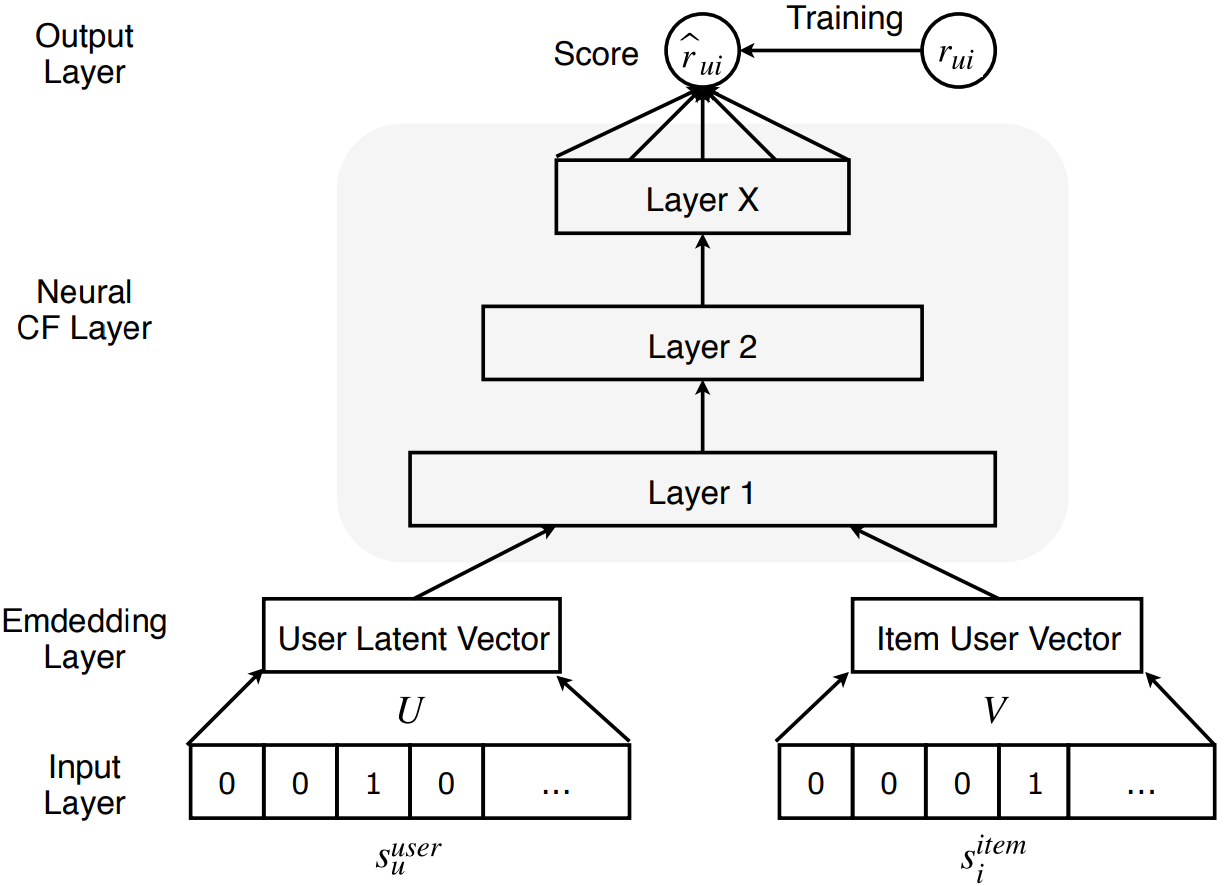
\includegraphics[width=5.7cm]{MusicRecomSurvey/pics/neumf.png}
\centering{(a)}
\end{minipage}
\hspace{1cm}
\begin{minipage}[t]{6.0cm}
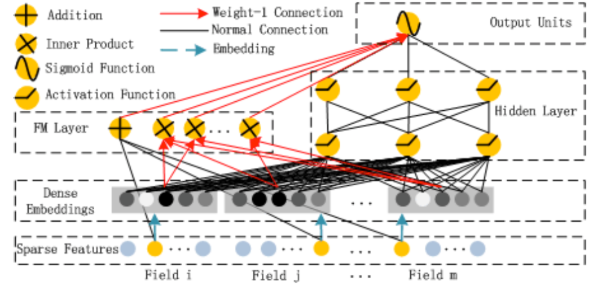
\includegraphics[width=6.0cm]{MusicRecomSurvey/pics/DeepFM.png}
\centering{(b)}
\end{minipage}
\caption{(a) Neural Collaborative Filtering; (b) Deep Factorization Machine.}
%\label{fig:windowsize}
\label{fig:ncf}
\end{center}
\end{figure}
\paragraph{Neural Collaborative Filtering(NCF)\cite{he2017neural}}
此方法改进了传统的协同过滤方法,通过MLP引入了非线性关系,能够更好地从用户评价矩阵中提取出用户、物品本身的特征。

记$s_{u}^{u s e r}$ 和 $s_{i}^{i t e m}$ 分别代表单边信息(如用户个人信息、物品特征),或者用户物品ID的one-hot编码。评分函数定义为:
    
\begin{equation}
\hat{r}_{u i}=f\left(U^{T} \cdot s_{u}^{u s e r}, V^{T} \cdot s_{i}^{i t e m} | U, V, \theta\right)
\end{equation}
    
    其中,f代表着多层感知机,$\theta$ 为网络的参数。对应loss为
    
    \begin{equation}
\mathcal{L}=-\sum_{(u, i) \in O \cup \mathcal{O}^{-}} r_{u i} \log \hat{r}_{u i}+\left(1-r_{u i}\right) \log \left(1-\hat{r}_{u i}\right)
\end{equation}
    
    \cite{lian2017cccfnet}引入multi-view拓展了NCF模型,适用于跨模态推荐。
    
    \cite{he2018outer}提出ConvNCF,使用CNN扩展NCF模型。它采用外积而不是内积来给用户物品关系建模,数据通过外积之后,进入CNN,能捕捉到嵌入层高阶的相关性。
    
    \cite{zhang2018neurec}发现,可以使用用户评价矩阵中的行和列来替代用户或物品的ID编码作为输入,这样可以保留用户-物品关系的相似性。
    
    有些工作\cite{niu2018neural}更换损失函数为pairwise ranking loss,来提高模型表现。

   
\paragraph{Deep Factorization Machine(DeepFM)\cite{guo2017deepfm}}
此方法拓展了传统的FM方法,将Factorization Machine 与 MLP 相结合,能够通过深度神经网络学习高阶的特征关系,通过FM学习低阶的特征关系。

DeepFM使用wide\& deep \cite{cheng2016wide}的框架,将wide部分替换为FM层。

\begin{equation}
y_{\mathrm{FM}}=\langle W, X\rangle+\sum_{i}^{n} \sum_{j=i+1}^{n}\left\langle v_{i}, v_{j}\right\rangle x_{i} x_{j}
\end{equation}
\begin{equation}
y_{\mathrm{MLP}}=\sigma\left(W^{(H+1)} a^{H}+b^{(H+1)}\right)
\end{equation}
\begin{equation}
\hat{r}_{u i}=\sigma\left(y_{F M}(x)+y_{M L P}(x)\right)
\end{equation}

输入是特征ID,通过Embeddings层得到稠密编码,同时进入FM层和MLP层联合训练。

\cite{lian2018xdeepfm}通过十分深的FM来联合训练显式和隐式的特征关系。

\cite{he2017neural}将二阶交互项替换为MLP,并且使用dropout和batch normalization 提升模型效果。

 \paragraph{Multi-View Deep Neural Network (MV-DNN)\cite{elkahky2015multi}}
\begin{figure}
\begin{center}
\begin{minipage}[t]{5.7cm}
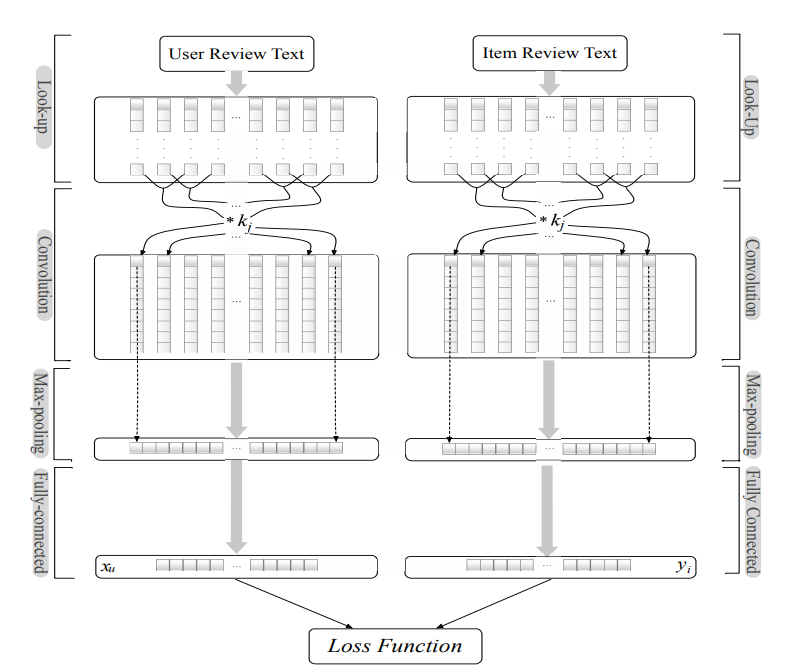
\includegraphics[width=5.7cm]{MusicRecomSurvey/pics/deepconn.png}
\centering{(a)}
\end{minipage}
\hspace{1cm}
\begin{minipage}[t]{6.0cm}
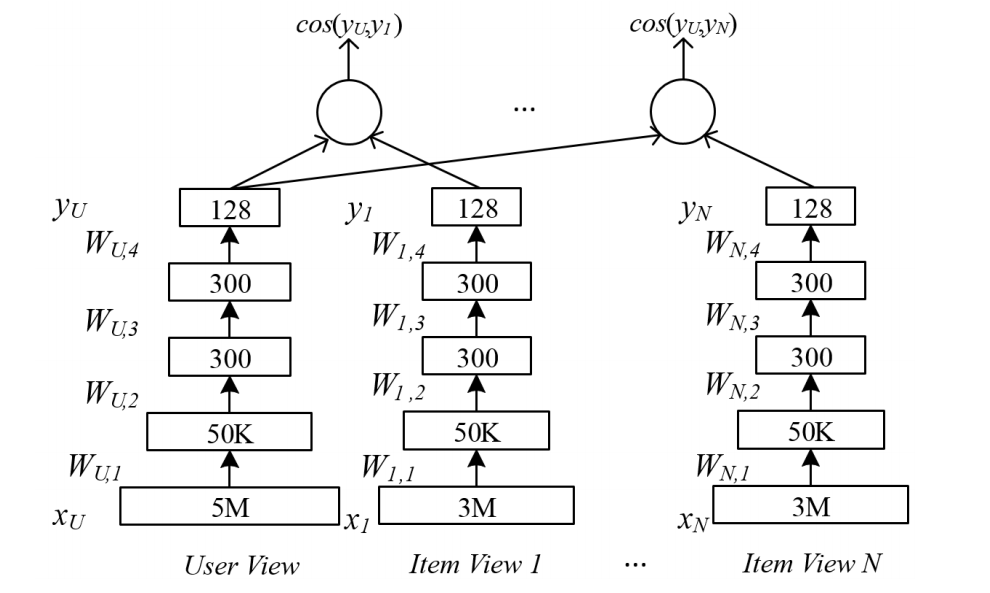
\includegraphics[width=6.0cm]{MusicRecomSurvey/pics/MVDNN2.png}
\centering{(b)}
\end{minipage}
\caption{(a) DeepCoNN; (b) Multi-View DNN.}
%\label{fig:windowsize}
\label{fig:deepconn}
\end{center}
\end{figure}
Multi-View Deep Neural Network (MV-DNN)是设计跨模态推荐系统的算法,将user信息作为pivot view,将所有其他域的信息(Z domains)作为auxiliary view,根据Z对user-domain的信息得到Z个评分。其损失函数为:
\begin{equation}
\mathcal{L}=\underset{\theta}{\operatorname{argmin}} \sum_{j=1}^{Z} \frac{\exp \left(\gamma \cdot \operatorname{cosine}\left(Y_{u}, Y_{a, j}\right)\right)}{\sum_{X^{\prime} \in R^{d a}} \exp \left(\gamma \cdot \operatorname{cosine}\left(Y_{u}, f_{a}\left(X^{\prime}\right)\right)\right)}
\end{equation}
其中$\theta$为模型参数, $\gamma$为平滑因子, $Y_{u}$ 是user view的输出, $a$ 是active view的编号。$R^{d a}$ 是view $a$对应的输入域 。 

MV-DNN 能够扩展到多个域,但是它基于一个假设——一个域中有类似偏好的用户,在其他领域偏好也类似。 直觉上,这个假设在许多情况下并不适用,因此,可以引入不同邻域的相关性等先验知识来缓解这个问题。


\subsubsection{用户序列建模}
\begin{figure}
\begin{center}
\begin{minipage}[t]{5.7cm}
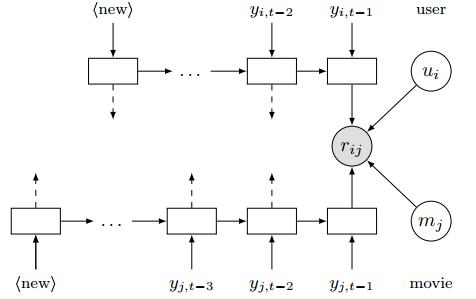
\includegraphics[width=5.7cm]{MusicRecomSurvey/pics/rrnb.png}
\centering{(a)RRN模型示意}
\end{minipage}
\hspace{1cm}
\begin{minipage}[t]{6.0cm}
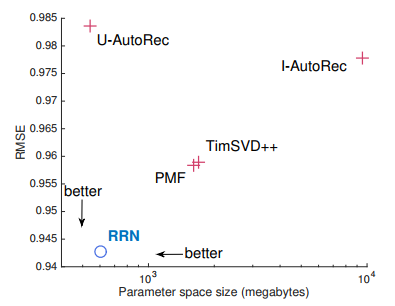
\includegraphics[width=6.0cm]{MusicRecomSurvey/pics/result.png}
\centering{(b)RNN在6个月Netflix数据集上的准确率和模型大小}
\end{minipage}
\caption{Recurrent Recommender Networks}
%\label{fig:windowsize}
\label{fig:rrn}
\end{center}
\end{figure}
上述模型或者方法中,都假定用户偏好或者物品属性不会随时间改变,但是这个假设是不符合实际的。在实际世界中,物品属性本身会发生变化(如某些音乐由于符合社会思潮而变得受欢迎),时间会对用户/物品交互关系直接产生变化(如在圣诞节,人们更可能听关于圣诞主题的音乐),用户自身兴趣也会随时间变化(如孩子长大成人,可能不再常听儿童乐)。

Recurrent Recommender Network(RRN)\cite{wu2017recurrent}采用自回归模型的框架,利用LSTM来学习序列相关的信息。隐变量自回归模型可以描述为:
\begin{equation}
\hat{z}_{t+1}=f\left(h_{t}, z_{t}\right) \text { and } h_{t+1}=g\left(h_{t}, z_{t+1}\right)
\end{equation}

其中$z$为观测状态,$\hat{z}$为状态估计,$h$为隐变量,下标$t$为时间。

RRN中记$u_{i}$ 和 $m_{j}$分别为用户$i$和电影
$j$。为了解决动态变化的问题,引入时间下标,也即$u_{i t}$ 和$m_{j t}$。套用隐变量自回归方程,定义更新函数:

\begin{equation}
\begin{aligned} \hat{r}_{i j | t}=f\left(u_{i t}, m_{j t}\right) \text { and } u_{i, t+1} &=g\left(u_{i t},\left\{r_{i j | t}\right\}\right) \\ m_{j, t+1} &=h\left(m_{j t},\left\{r_{i j | t}\right\}\right) \end{aligned}
\end{equation}

其中$\hat{r}_{i j | t}$ 代表用户 $i$对电影
$j$的评分预测,$r_{i j | t}$ 是在时间 $t $的实际评分。函数$f, g$ 和 $h$ 通过训练得到。

模型中$g$与LSTM相关,训练中调整LSTM的参数以调整g;考虑到用户/物品本身既有稳定的属性,也有随时间改变的特点,$f$函数分为两部分:
\begin{equation}
\hat{r}_{i j | t}=f\left(u_{i t}, m_{j t}, u_{i}, m_{j}\right) :=\left\langle\tilde{u}_{i t}, \tilde{m}_{j t}\right\rangle+\left\langle u_{i}, m_{j}\right\rangle
\end{equation}
\begin{equation}
\tilde{u}_{i t}=W_{\mathrm{user}} u_{i t}+b_{\mathrm{user}} \text { and } \tilde{m}_{j t}=W_{\mathrm{movie}} m_{j t}+b_{\mathrm{movie}}
\end{equation}

最终目标函数为:

\begin{equation}
\underset{\theta}{\operatorname{minimize}} \sum_{(i, j, t) \in \mathcal{I}_{\text { train }}}\left(r_{i j | t}-\hat{r}_{i j | t}(\theta)\right)^{2}+R(\theta)
\end{equation}

该模型采用subspace descent 的方法进行求解,也就是更新一个参数的同时,固定其他的参数。从图\ref{fig:rrn}可以看出,综合准确率与模型大小,对比了其他许多考虑了序列的模型,该模型展示出很大的提升。

\subsubsection{深度混合模型}
\paragraph{CNN 与 Autoencoder}
Collaborative Knowledge Based Embedding(CKE)\cite{zhang2016collaborative}将AE与CNN结合来做特征的提取。它通过不同的embedding技术,利用了结构化、文本、视觉内容的信息,采用TransR\cite{lin2015learning}来提取结构化信息,stacked convolutional auto-encoder(SCAE)来提取视觉信息。整个推荐的过程与CDL类似。
\paragraph{RNN 与 Autoencoder}
\cite{wang2016collaborative}提出融合RNN和denoising autoencoder来克服模型鲁棒性、文本序列化建模的问题。作者将自编码器的前馈网络中一些层替换为RNN层,使得编码器能够捕捉到物品内容的序列信息。作者通过wildcard denoising 和 beta-pooling 技术来避免模型过拟合。
\paragraph{RNN 与 Attention}
\cite{li2016hashtag}提出使用基于注意力机制的LSTM模型,来做推文话题的推荐。这个工作利用了RNN和注意力机制的优点,能够从微博中同时捕捉序列性质和信息量丰富的词语。
